\documentclass[12pt]{article}
\usepackage[utf8]{inputenc}
\usepackage{graphicx}
\usepackage{subcaption}
\usepackage{amsmath} 
\usepackage{fancyhdr} 
\usepackage{geometry} 
\usepackage{dirtytalk} 
\usepackage[english]{babel}
\usepackage{csquotes}
\usepackage{hyperref}
\usepackage{listings}
\lstset{
    language=C,
    basicstyle=\ttfamily, 
    numberstyle=\tiny,
    frame=single,
    breaklines=true,
}

\begin{document}
\begin{titlepage}
\begin{center}
    
\includegraphics[width=0.3\textwidth]{image.png} \\[0.2cm]
    
    \textbf{MINISTRY OF EDUCATION, CULTURE AND RESEARCH 
OF THE REPUBLIC OF MOLDOVA} \\[0.3cm]
    
    \textbf{Technical University of Moldova 
Faculty of Computers, Informatics and Microelectronics 
Department of Software and Automation Engineering} \\[2cm]
    
    \textbf{Postoronca Dumitru FAF-233}\\[0.5cm]
    
    \Huge \textbf{Report} \\[0.5cm]
    
    \large Laboratory Work №3\\[0.5cm]
    
    \textbf{of AA} \\[3cm]
    
    \begin{flushright}
        \textit{Checked by:} \\
        \textbf{Fistic Cristofor}, \textit{university assistant} \\
        DISA, FCIM, UTM
    \end{flushright}
    
    \vfill
    
    Chișinău -- 2024
\end{center}
\end{titlepage}


\newpage
\setcounter{page}{1}
\pagestyle{fancy}
\fancyhf{}
\rhead{\thepage}
\lhead{FAF-233 Postoronca Dumitru ; Laboratory work №3}

\section*{Conditions of the Task}
Empirical analysis of algorithms: Depth First Search (DFS), Breadth First Search(BFS)
\begin{enumerate}
    \item Implement the algorithms listed above in a programming language
    \item Establish the properties of the input data against which the analysis is performed
    \item Choose metrics for comparing algorithms
    \item Perform empirical analysis of the proposed algorithms
    \item Make a graphical presentation of the data obtained
    \item Make a conclusion on the work done.
\end{enumerate}

\clearpage
\section*{Input data}
\hspace{0.8cm}
To analyze and compare the sorting algorithms, we define the following input data conditions:
\begin{enumerate}
    \item Wideness of the graph(number of direct children):
      \begin{itemize}
        \item Small wideness (\textit{n} = 3)  
        \item Large wideness (\textit{n} = 20)  
      \end{itemize}

    \item Depth of the the graph:
      \begin{itemize}
        \item Low depth (\textit{d} = 3)  
        \item Big depth (\textit{d} = 11)
      \end{itemize}

    \item Edge Cases:
      \begin{itemize}
        \item All elements identical
        \item Cycled graph
        \item Some directed graphs
      \end{itemize}
\end{enumerate}

Input data was generated by a special function written in JS that takes as input 
the wideness of the graph (number of direct children each node will have) and it's depth.
Total number of nodes will be calculated by the formula: $$N_{nodes} = width^{depth}$$

\clearpage
\section*{Metrics in Algorithm analysis}

In this laboratory work I will try to test how each of the path finding algorithms work
depending on the width and the depth of graph. 

For this purpose I will run the same algorithm
to find the path to the node from the depth 1 down to the node which is the leaf.
In this way if the depth of generated graph is 5, I will show the metrics for: depth 1, 
depth 2, depth3, depth4, depth 5

\subsection*{Disabling Turbofan}
In order to perform the algorithm analysis I've written Javascript programs that would track the execution time of each algorithm
and run them in Node js. Node js uses V8 engine in order to execute the JavaScript programs. This engine consists of 2 components:
\begin{itemize}
  \item Interpreting machine Ignition\cite{bytecoderef}
  \item Optimizing compiler \textbf{Turbofan}, that can optimize and translate some of the JavaScript code into the machine code.

\end{itemize}
To reduce the influence of Turbofan on the validity of data, 
I have run the algorithms with \textit{--no-opt} flag to disable Turbofan.
This decision is motivated by the unpredictability of the optimizing compiler which can 
optimize the code for an algorithm with a long execution time and not optimize the efficient algorithm.
Thus I put all algorithms to equal execution conditions.

\subsection*{Algorithms Implementation}

\subsection*{Results}
After running of all the tests these are the results obtained:
\begin{figure}[h]
    \centering
    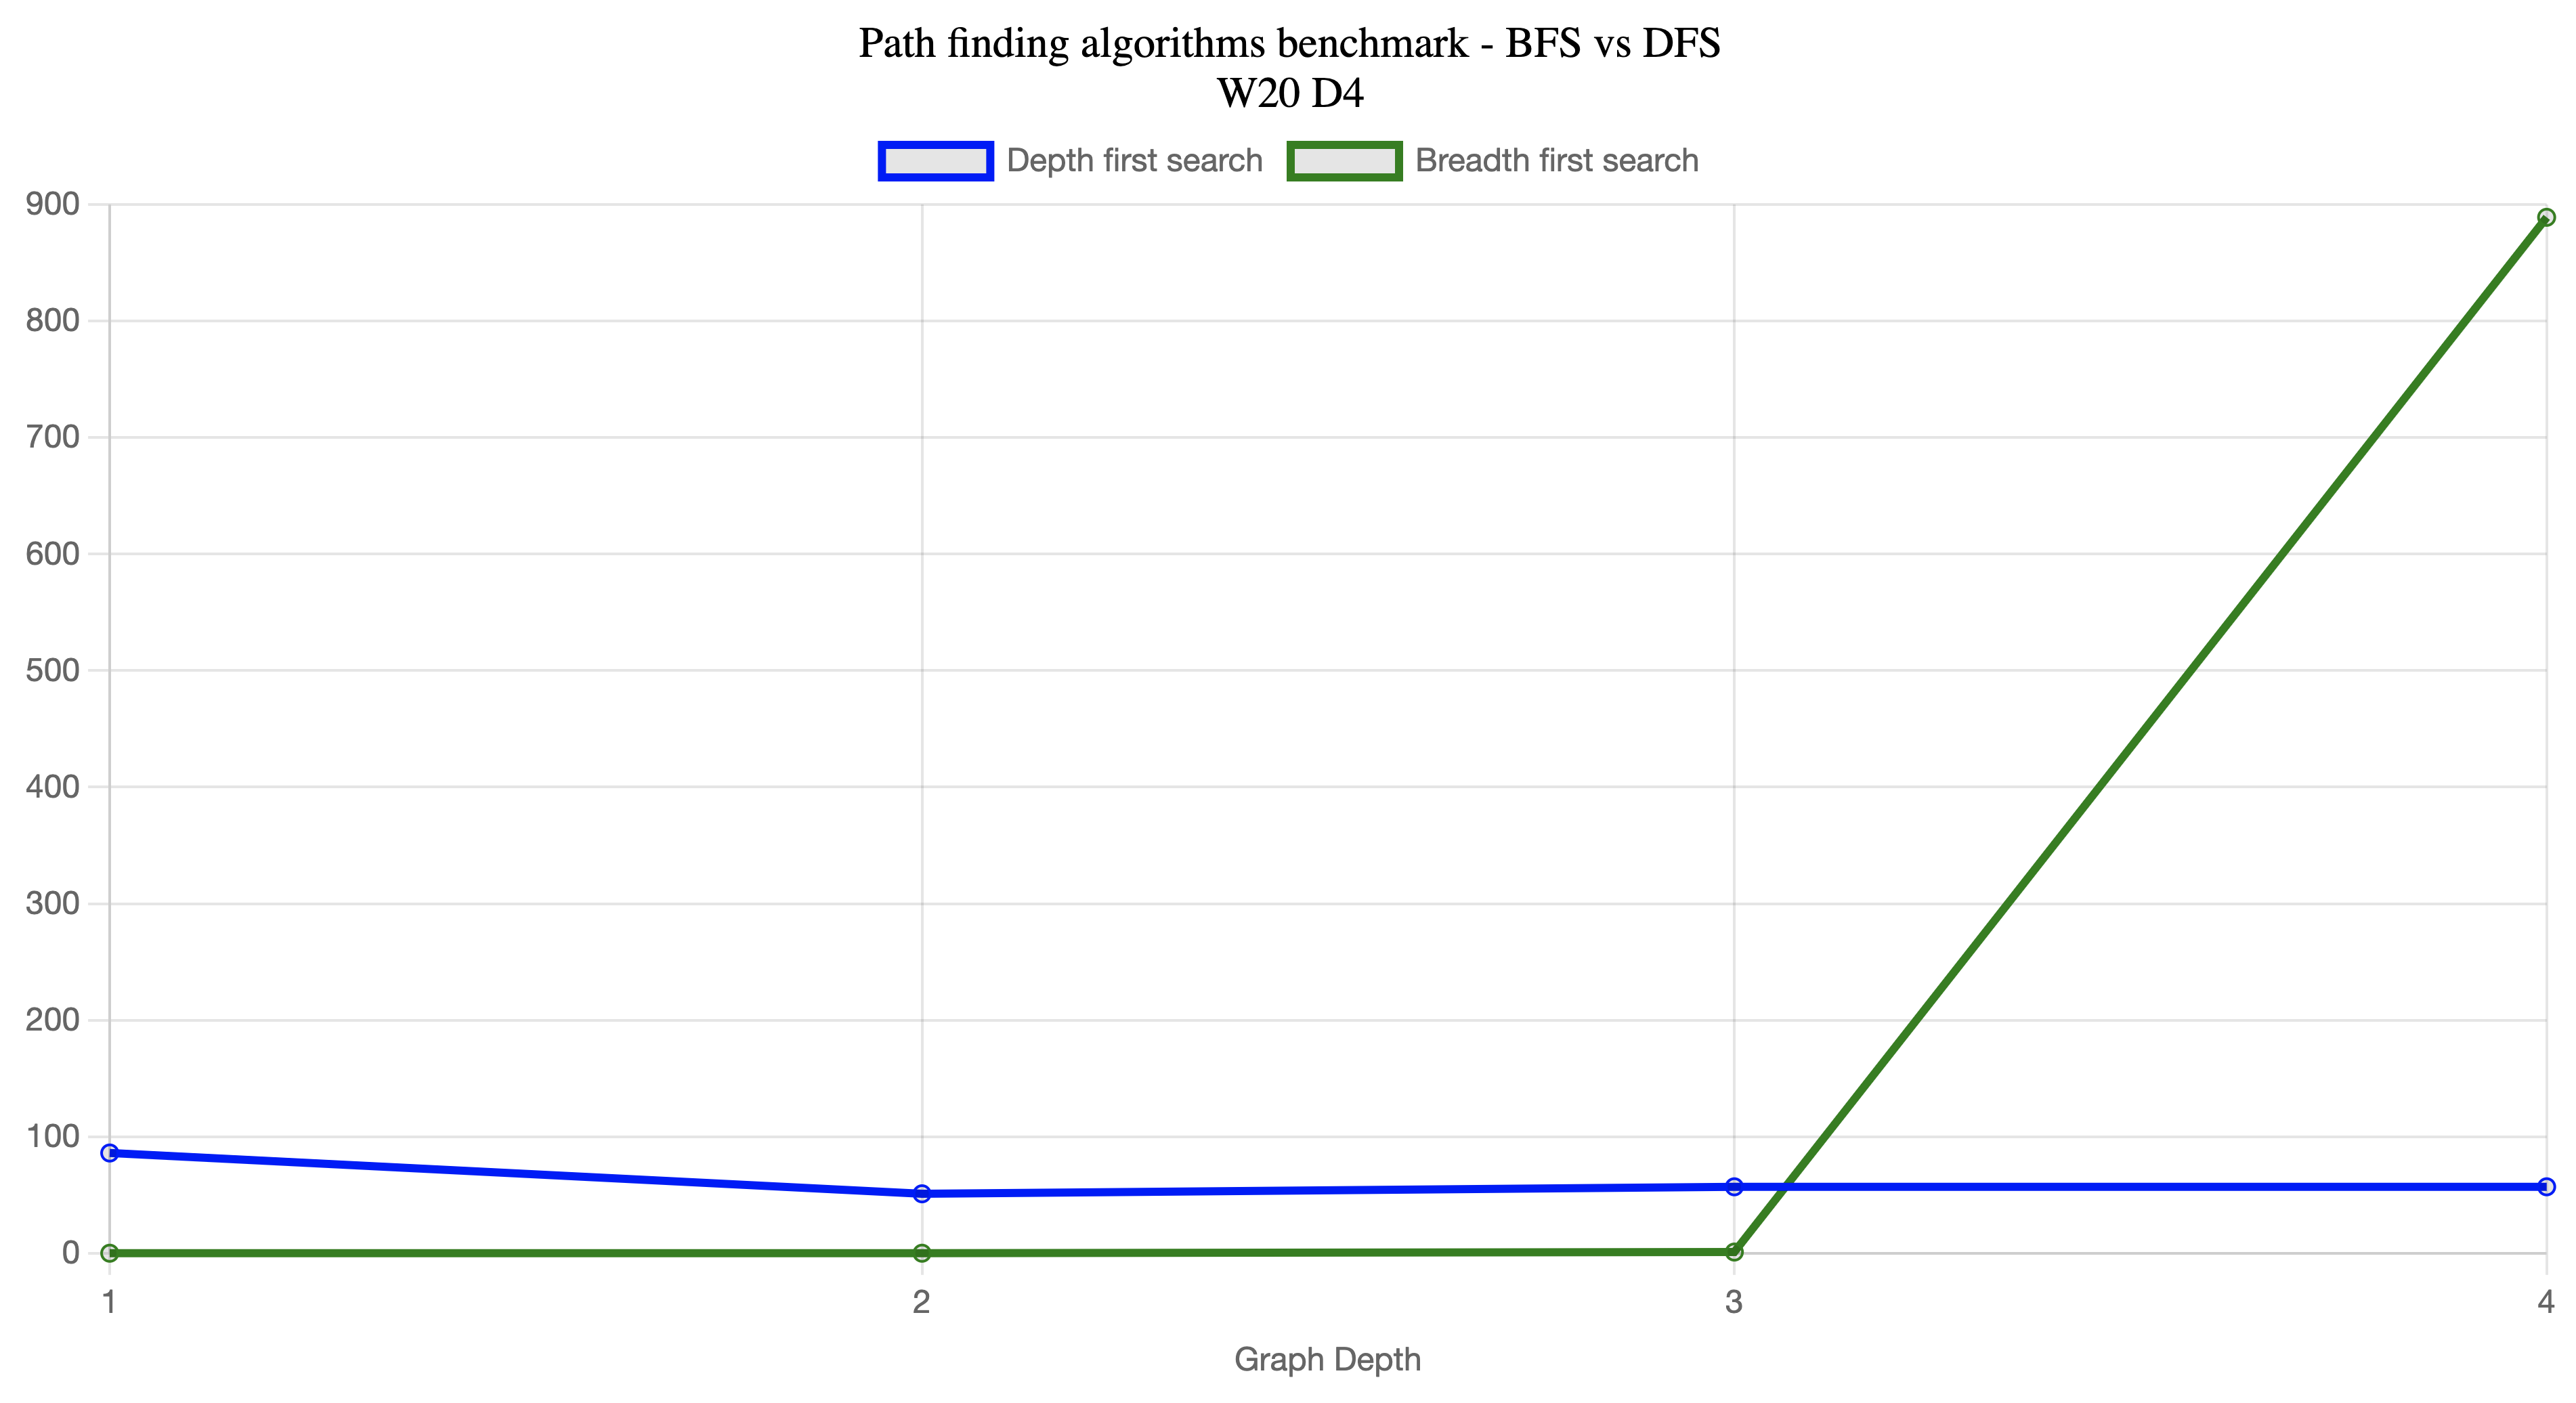
\includegraphics[width=1\textwidth]{images/w20d4.png}
    \caption{Path finding comparison for a graph with width 20 and depth 4}
    \label{fig:w20d4}
\end{figure}


\begin{figure}[h]
    \centering
    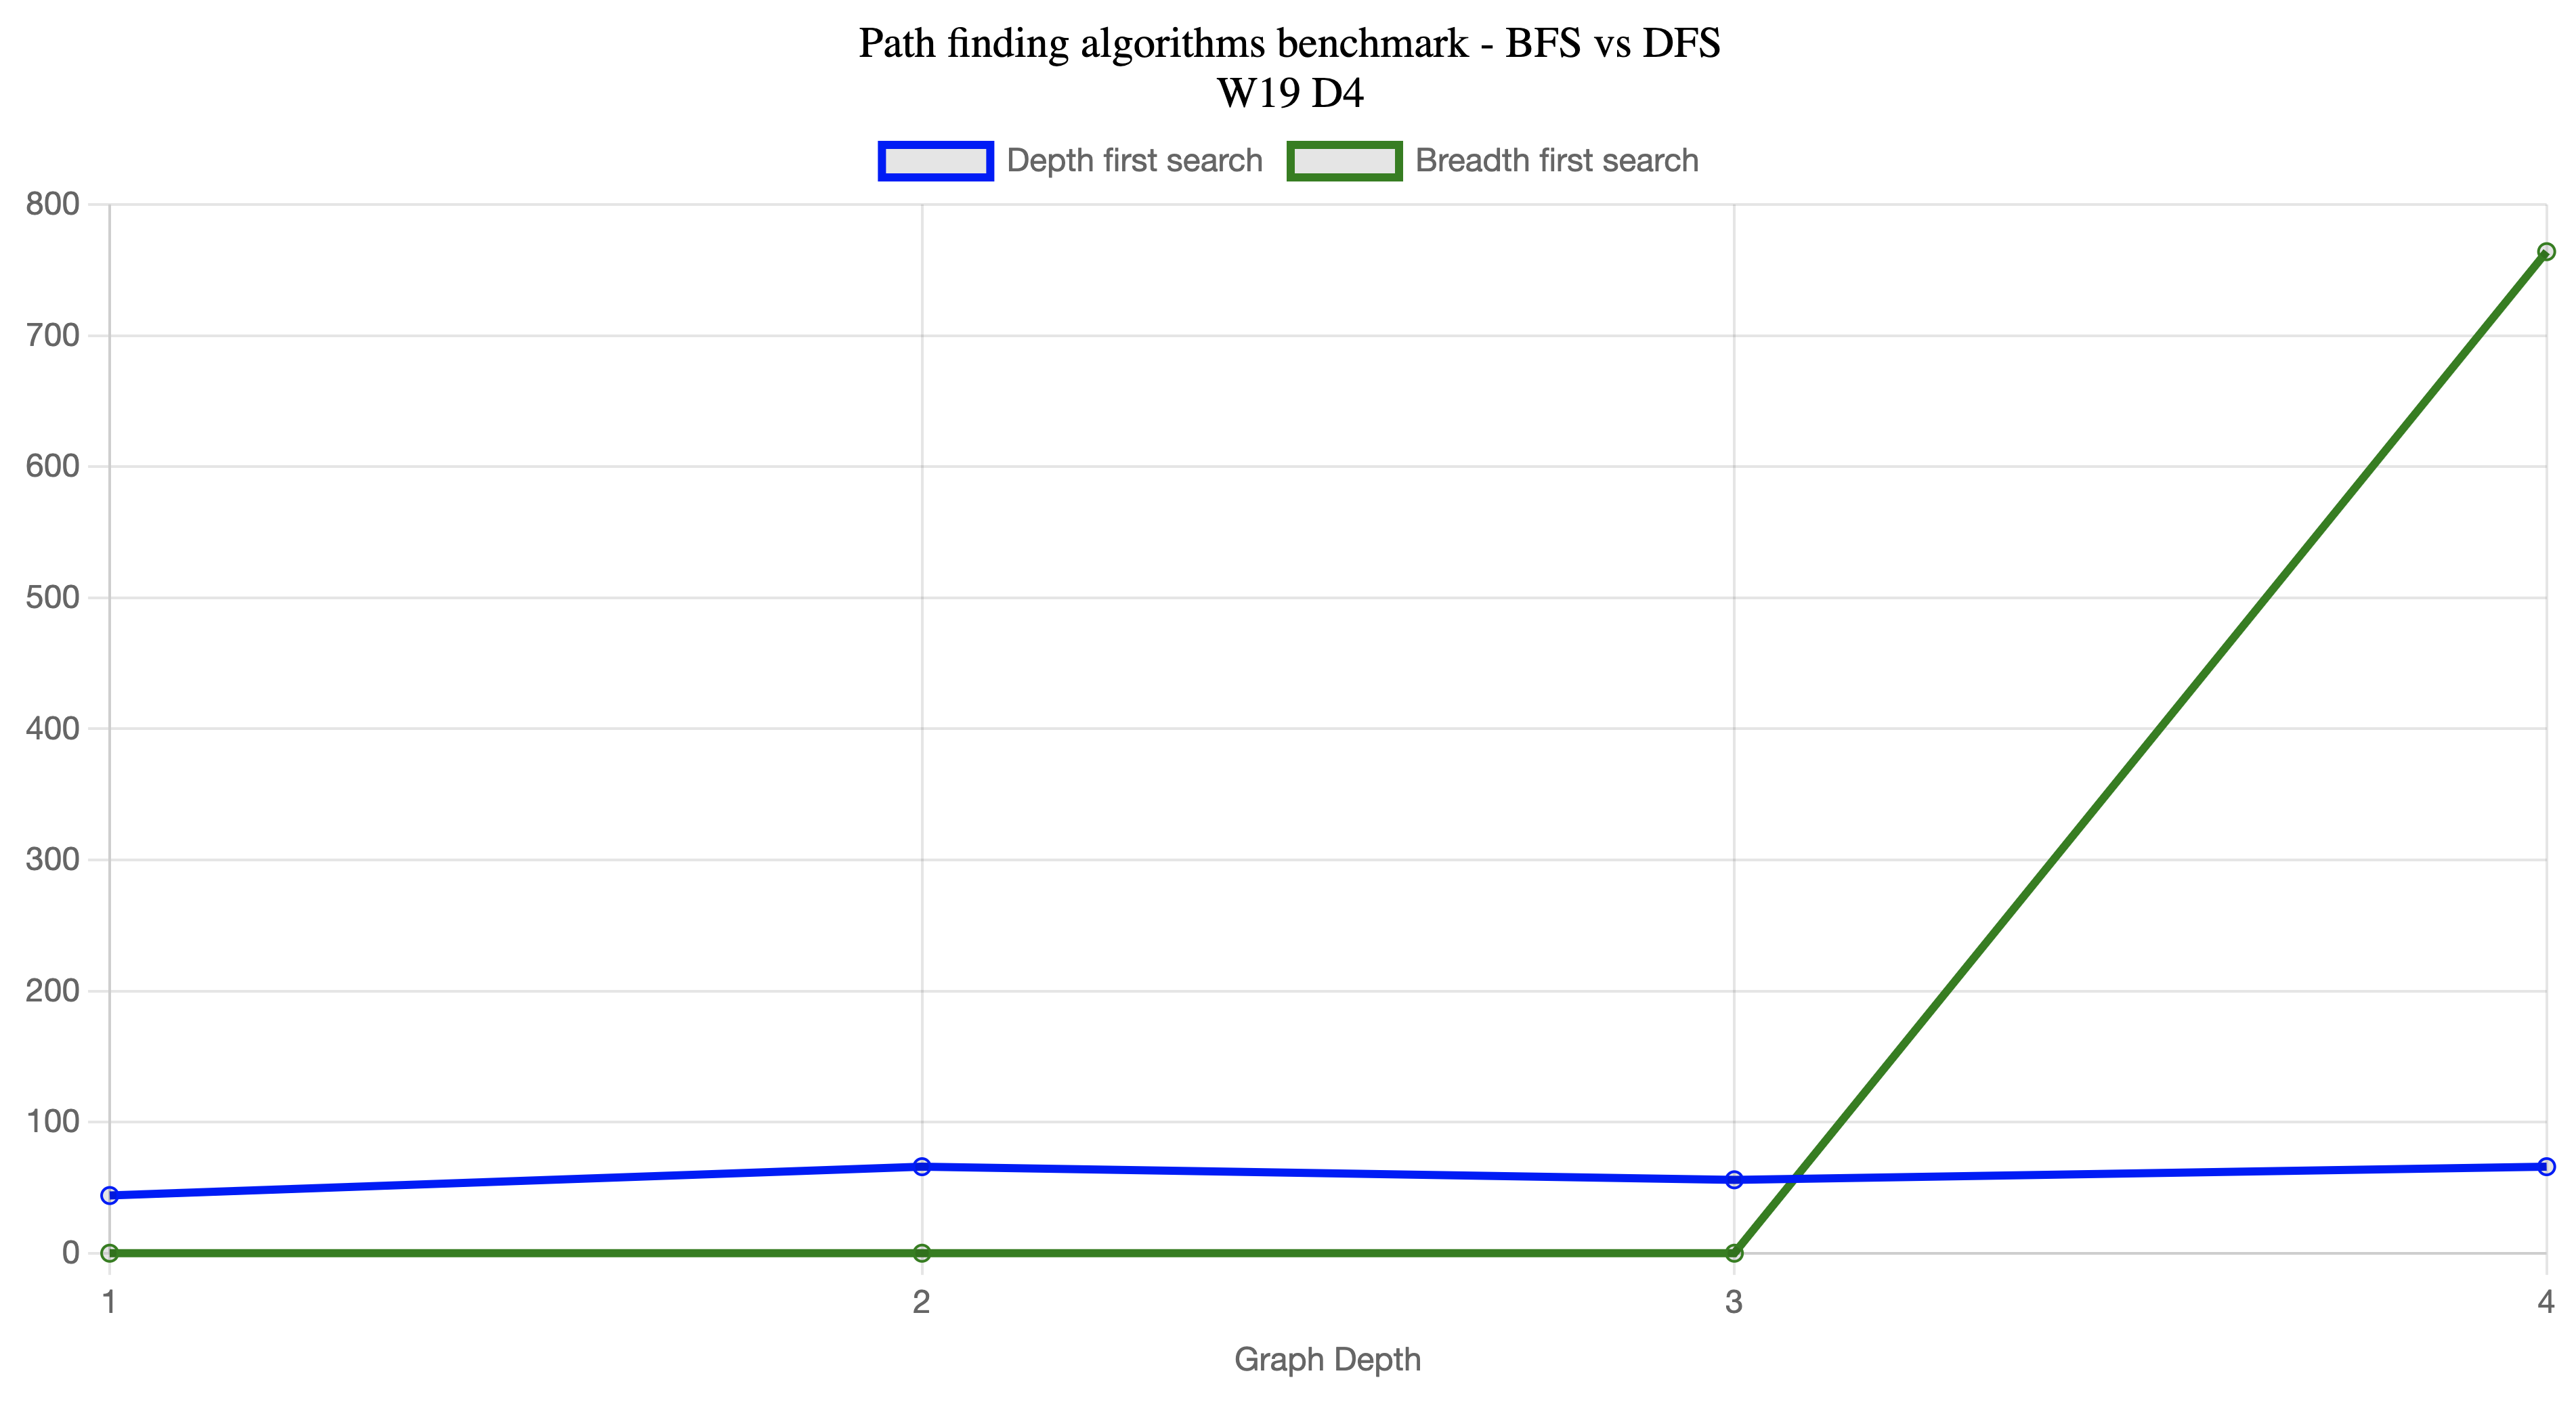
\includegraphics[width=1\textwidth]{images/w19d4.png}
    \caption{Path finding comparison for a graph with width 19 and depth 4}
    \label{fig:w19d4}
\end{figure}

\begin{figure}[h]
    \centering
    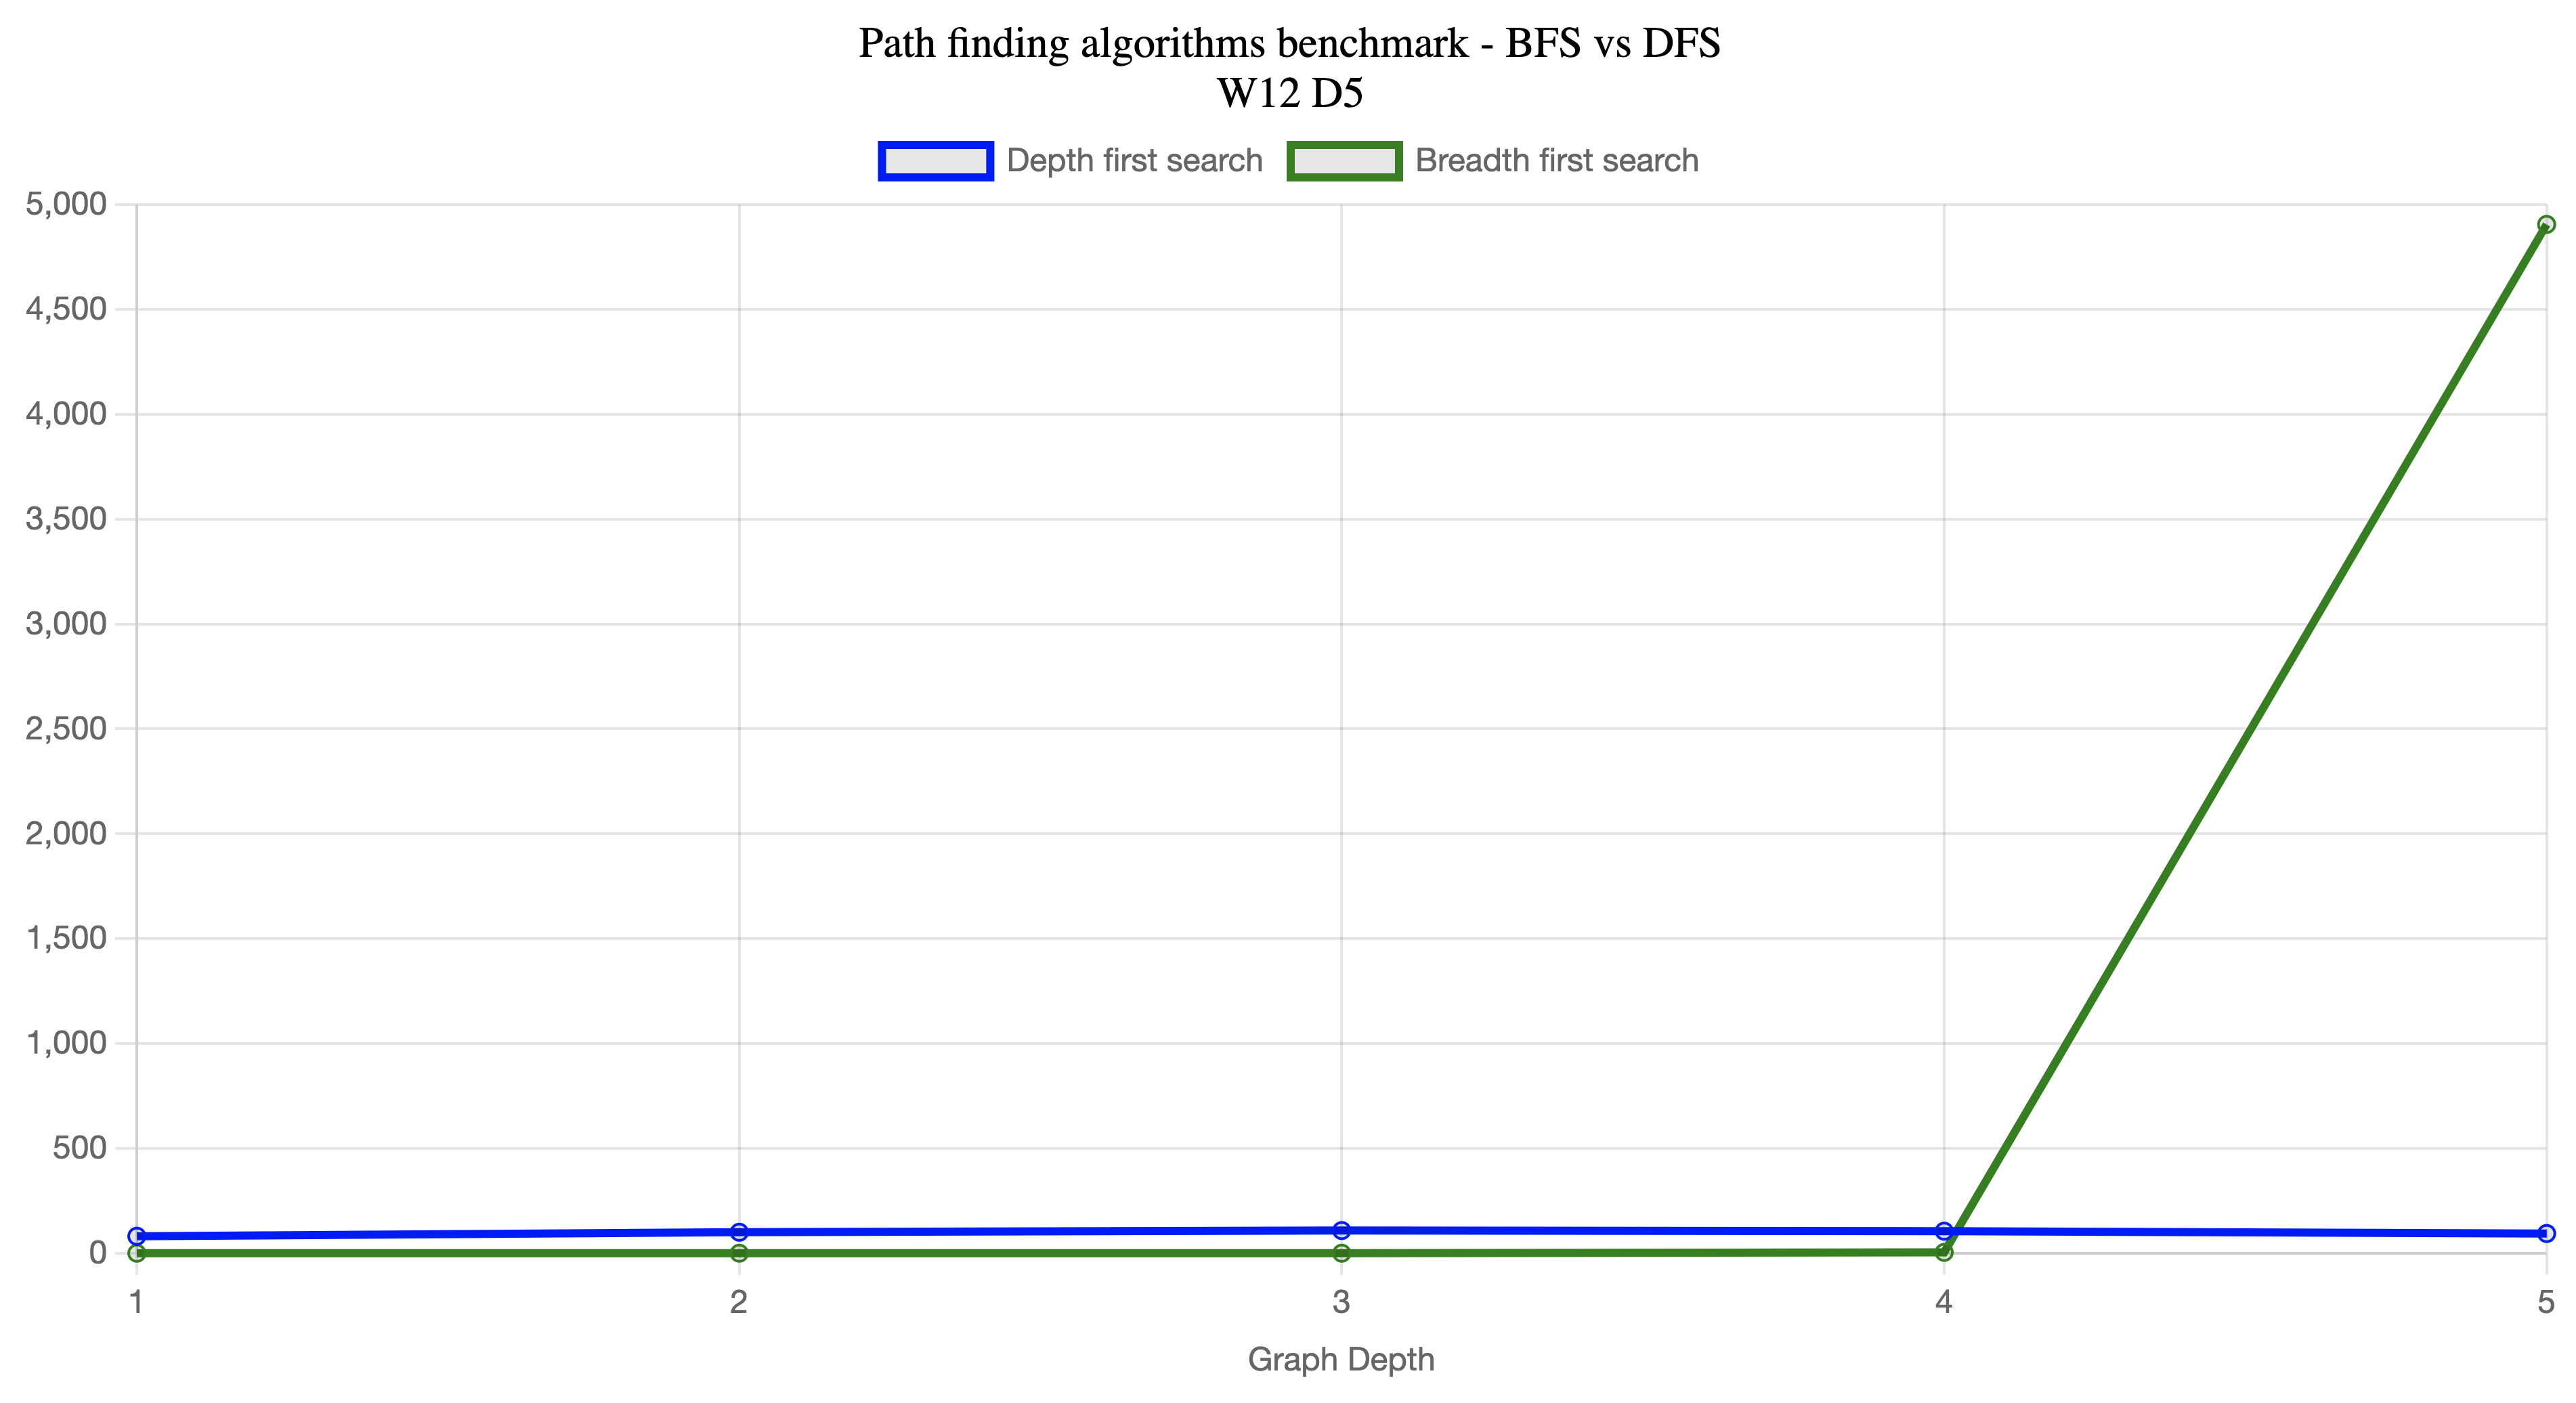
\includegraphics[width=1\textwidth]{images/w12d5.png}
    \caption{Path finding comparison for a graph with width 12 and depth 5}
    \label{fig:w12d5}
\end{figure}

\begin{figure}[h]
    \centering
    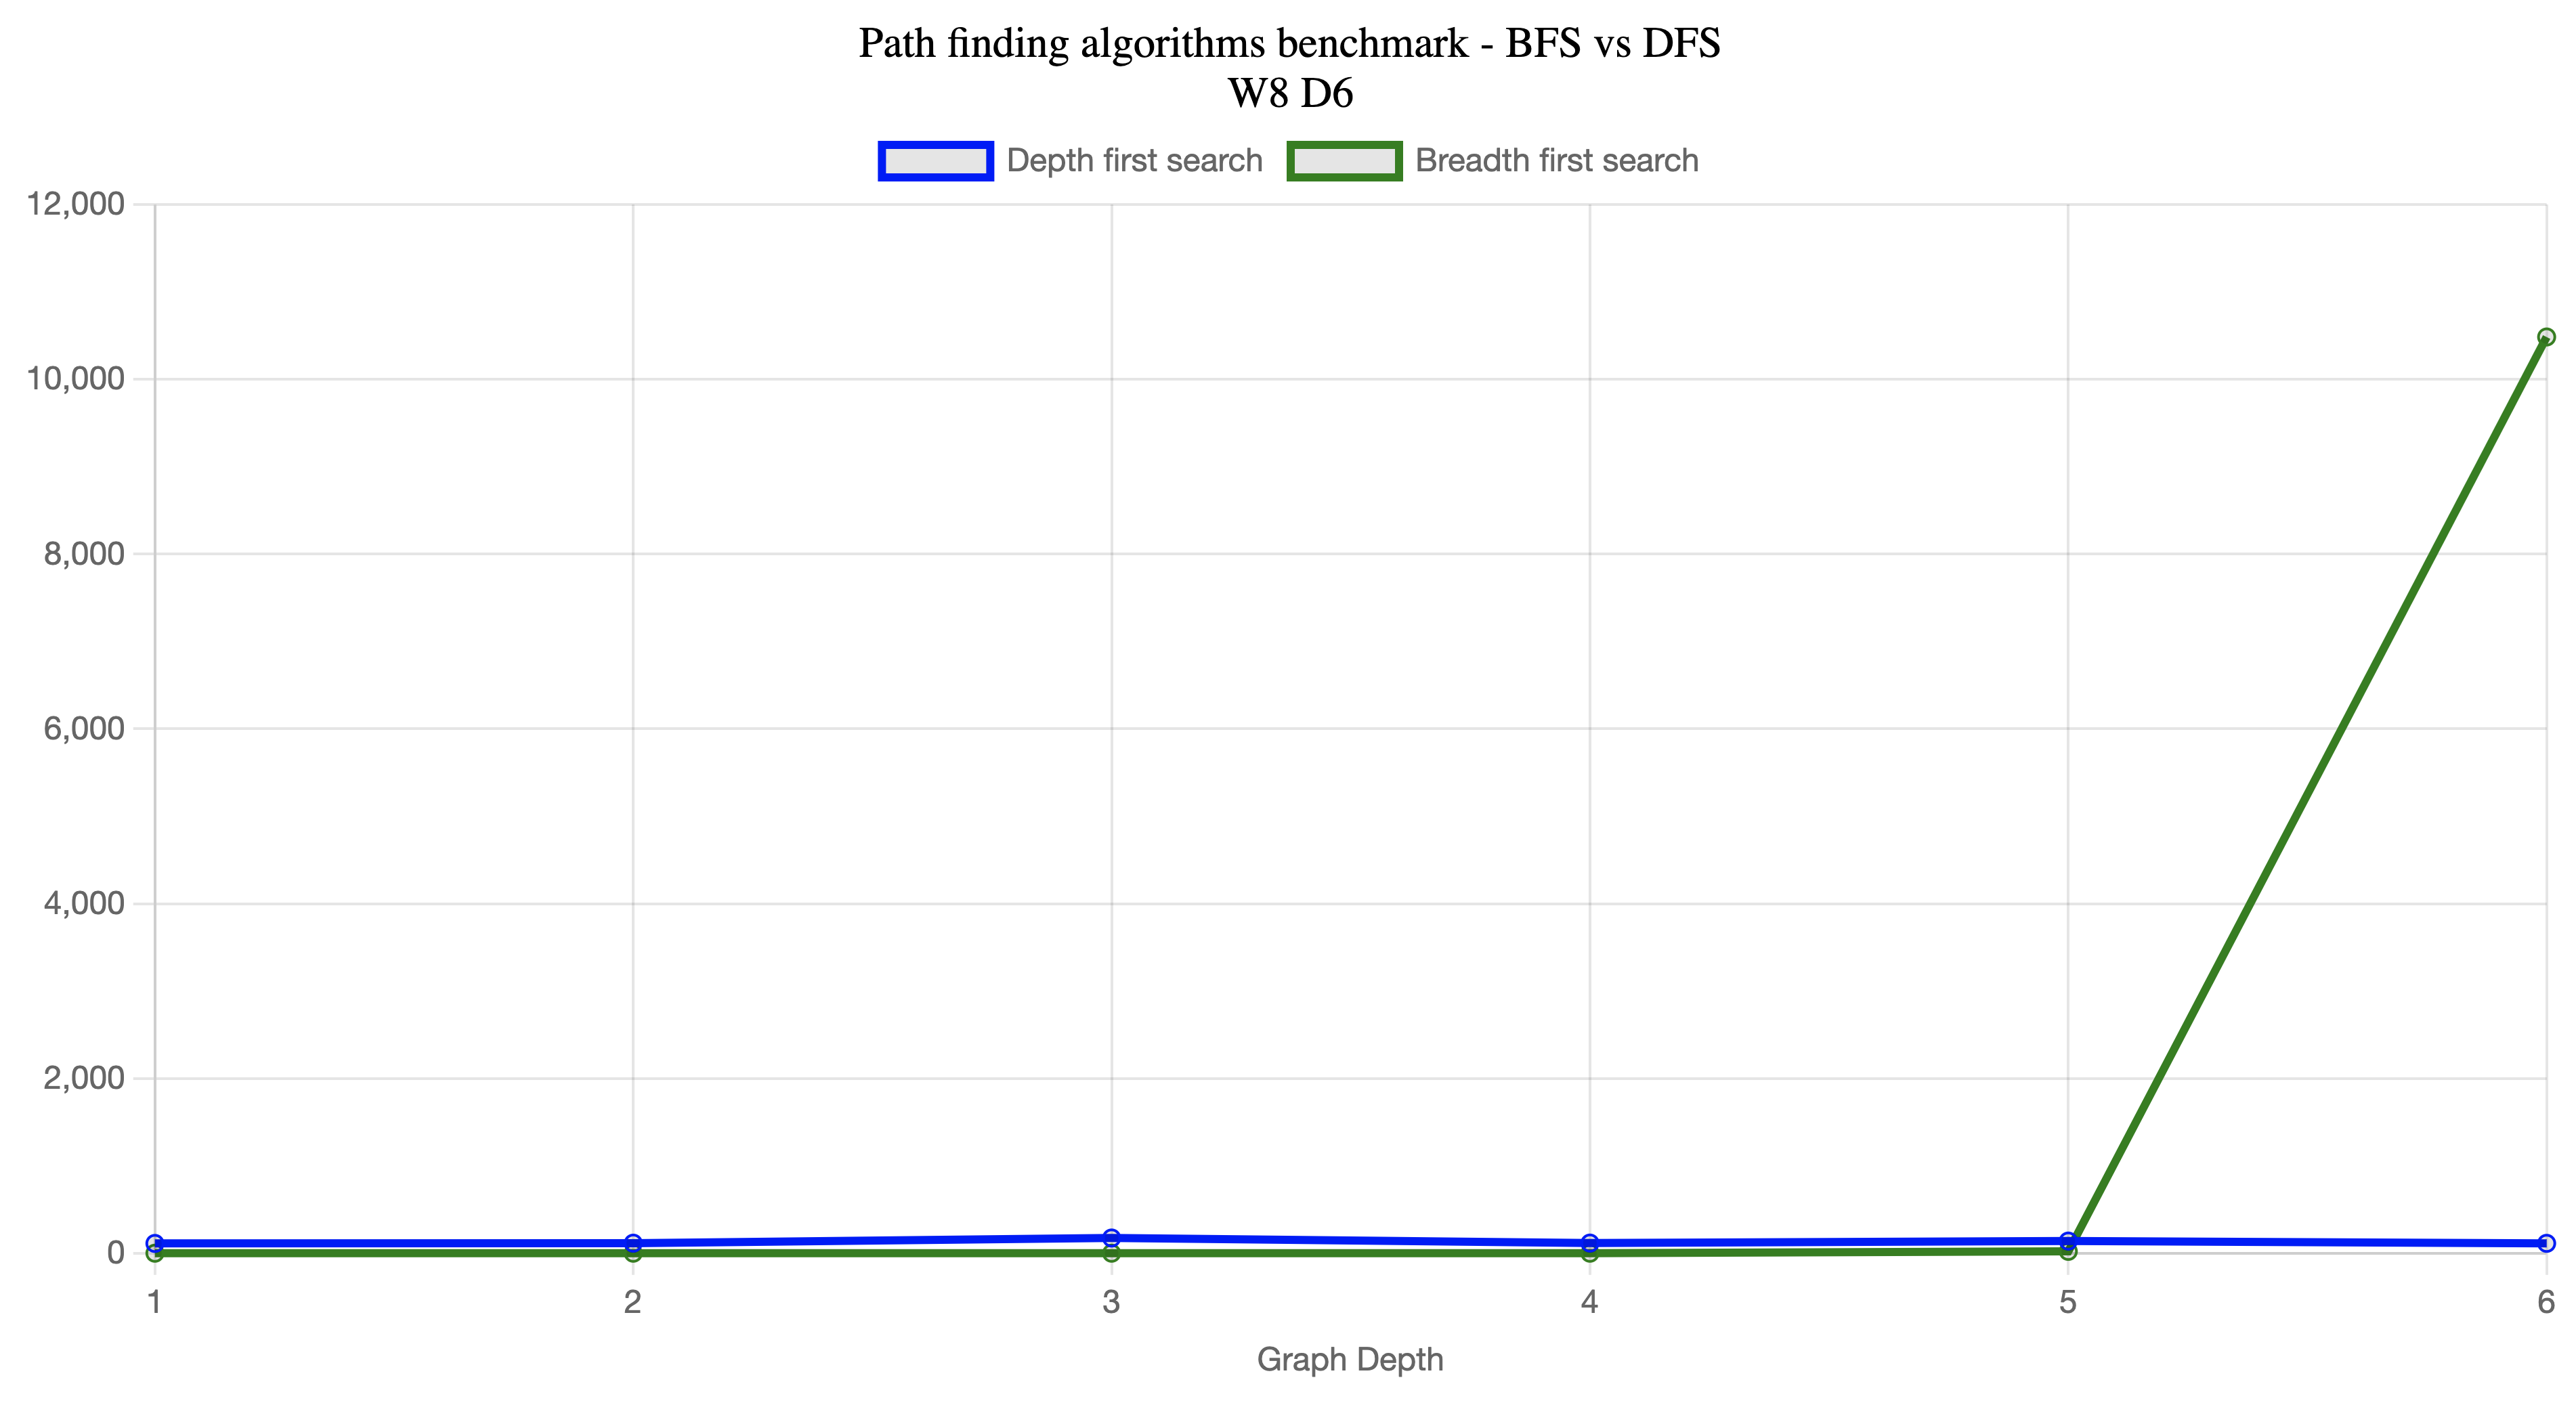
\includegraphics[width=1\textwidth]{images/w8d6.png}
    \caption{Path finding comparison for a graph with width 8 and depth 6}
    \label{fig:w8d6}
\end{figure}

\begin{figure}[h]
    \centering
    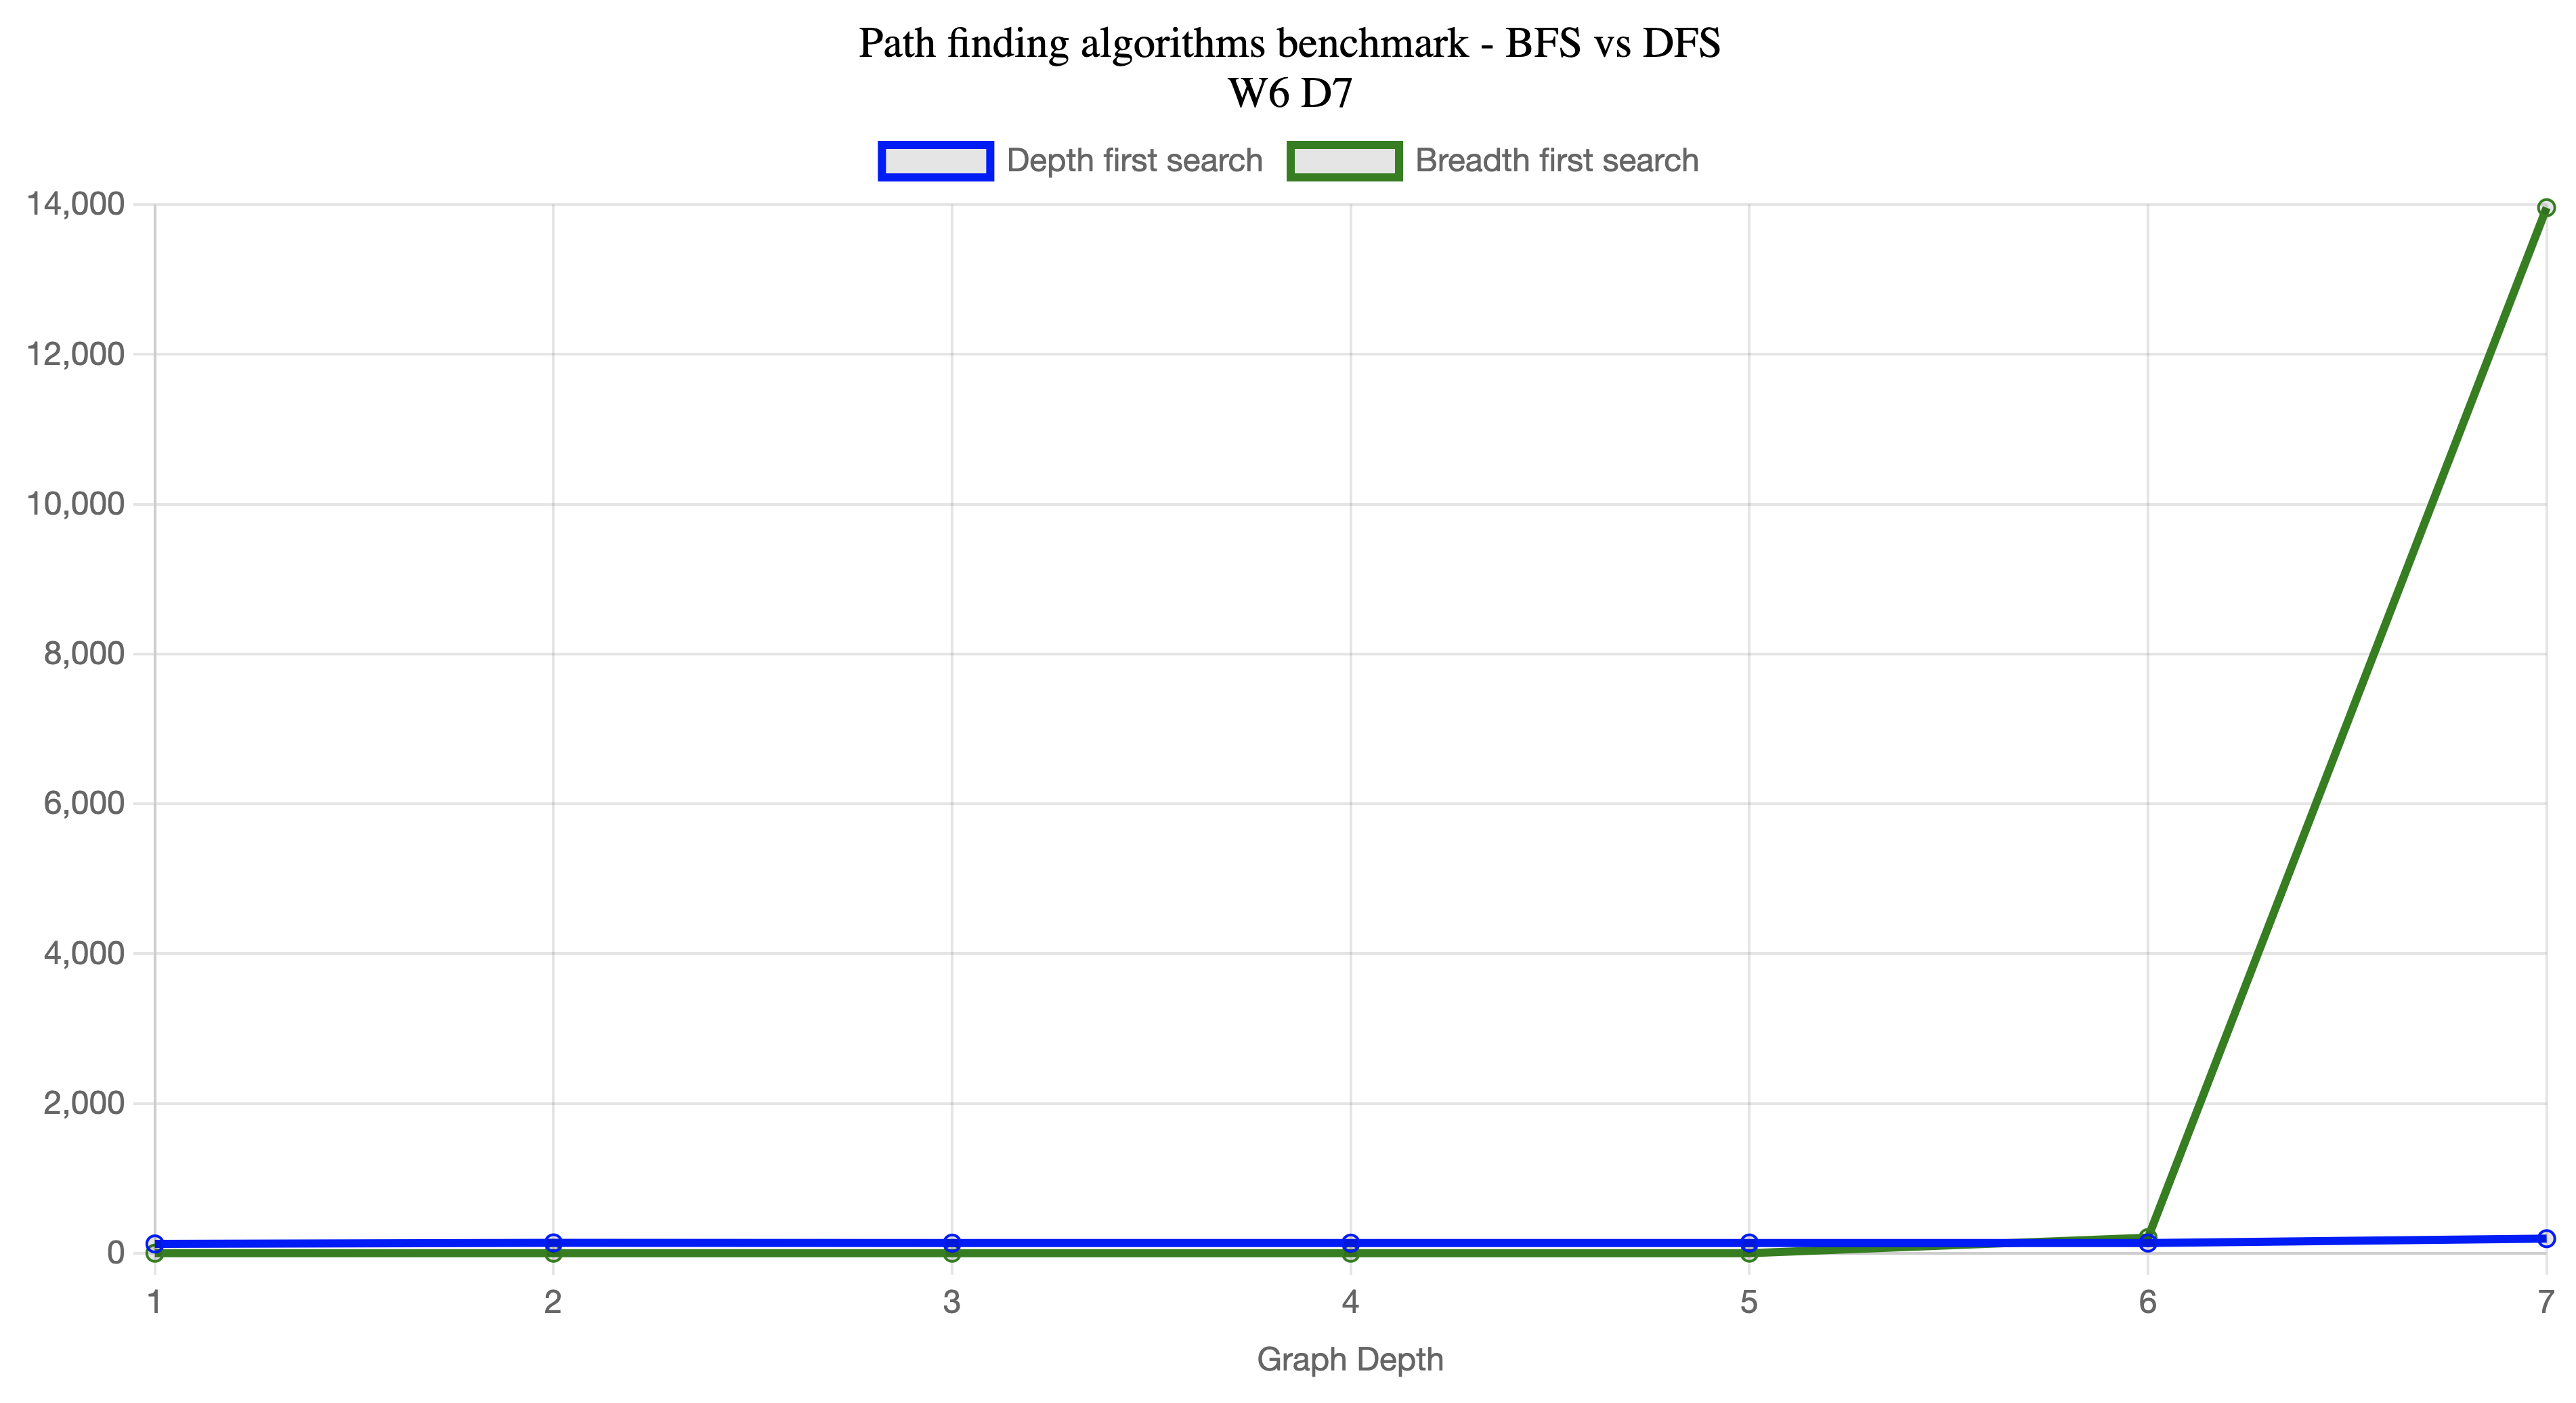
\includegraphics[width=1\textwidth]{images/w6d7.png}
    \caption{Path finding comparison for a graph with width 6 and depth 7}
    \label{fig:w6d7}
\end{figure}

\begin{figure}[h]
    \centering
    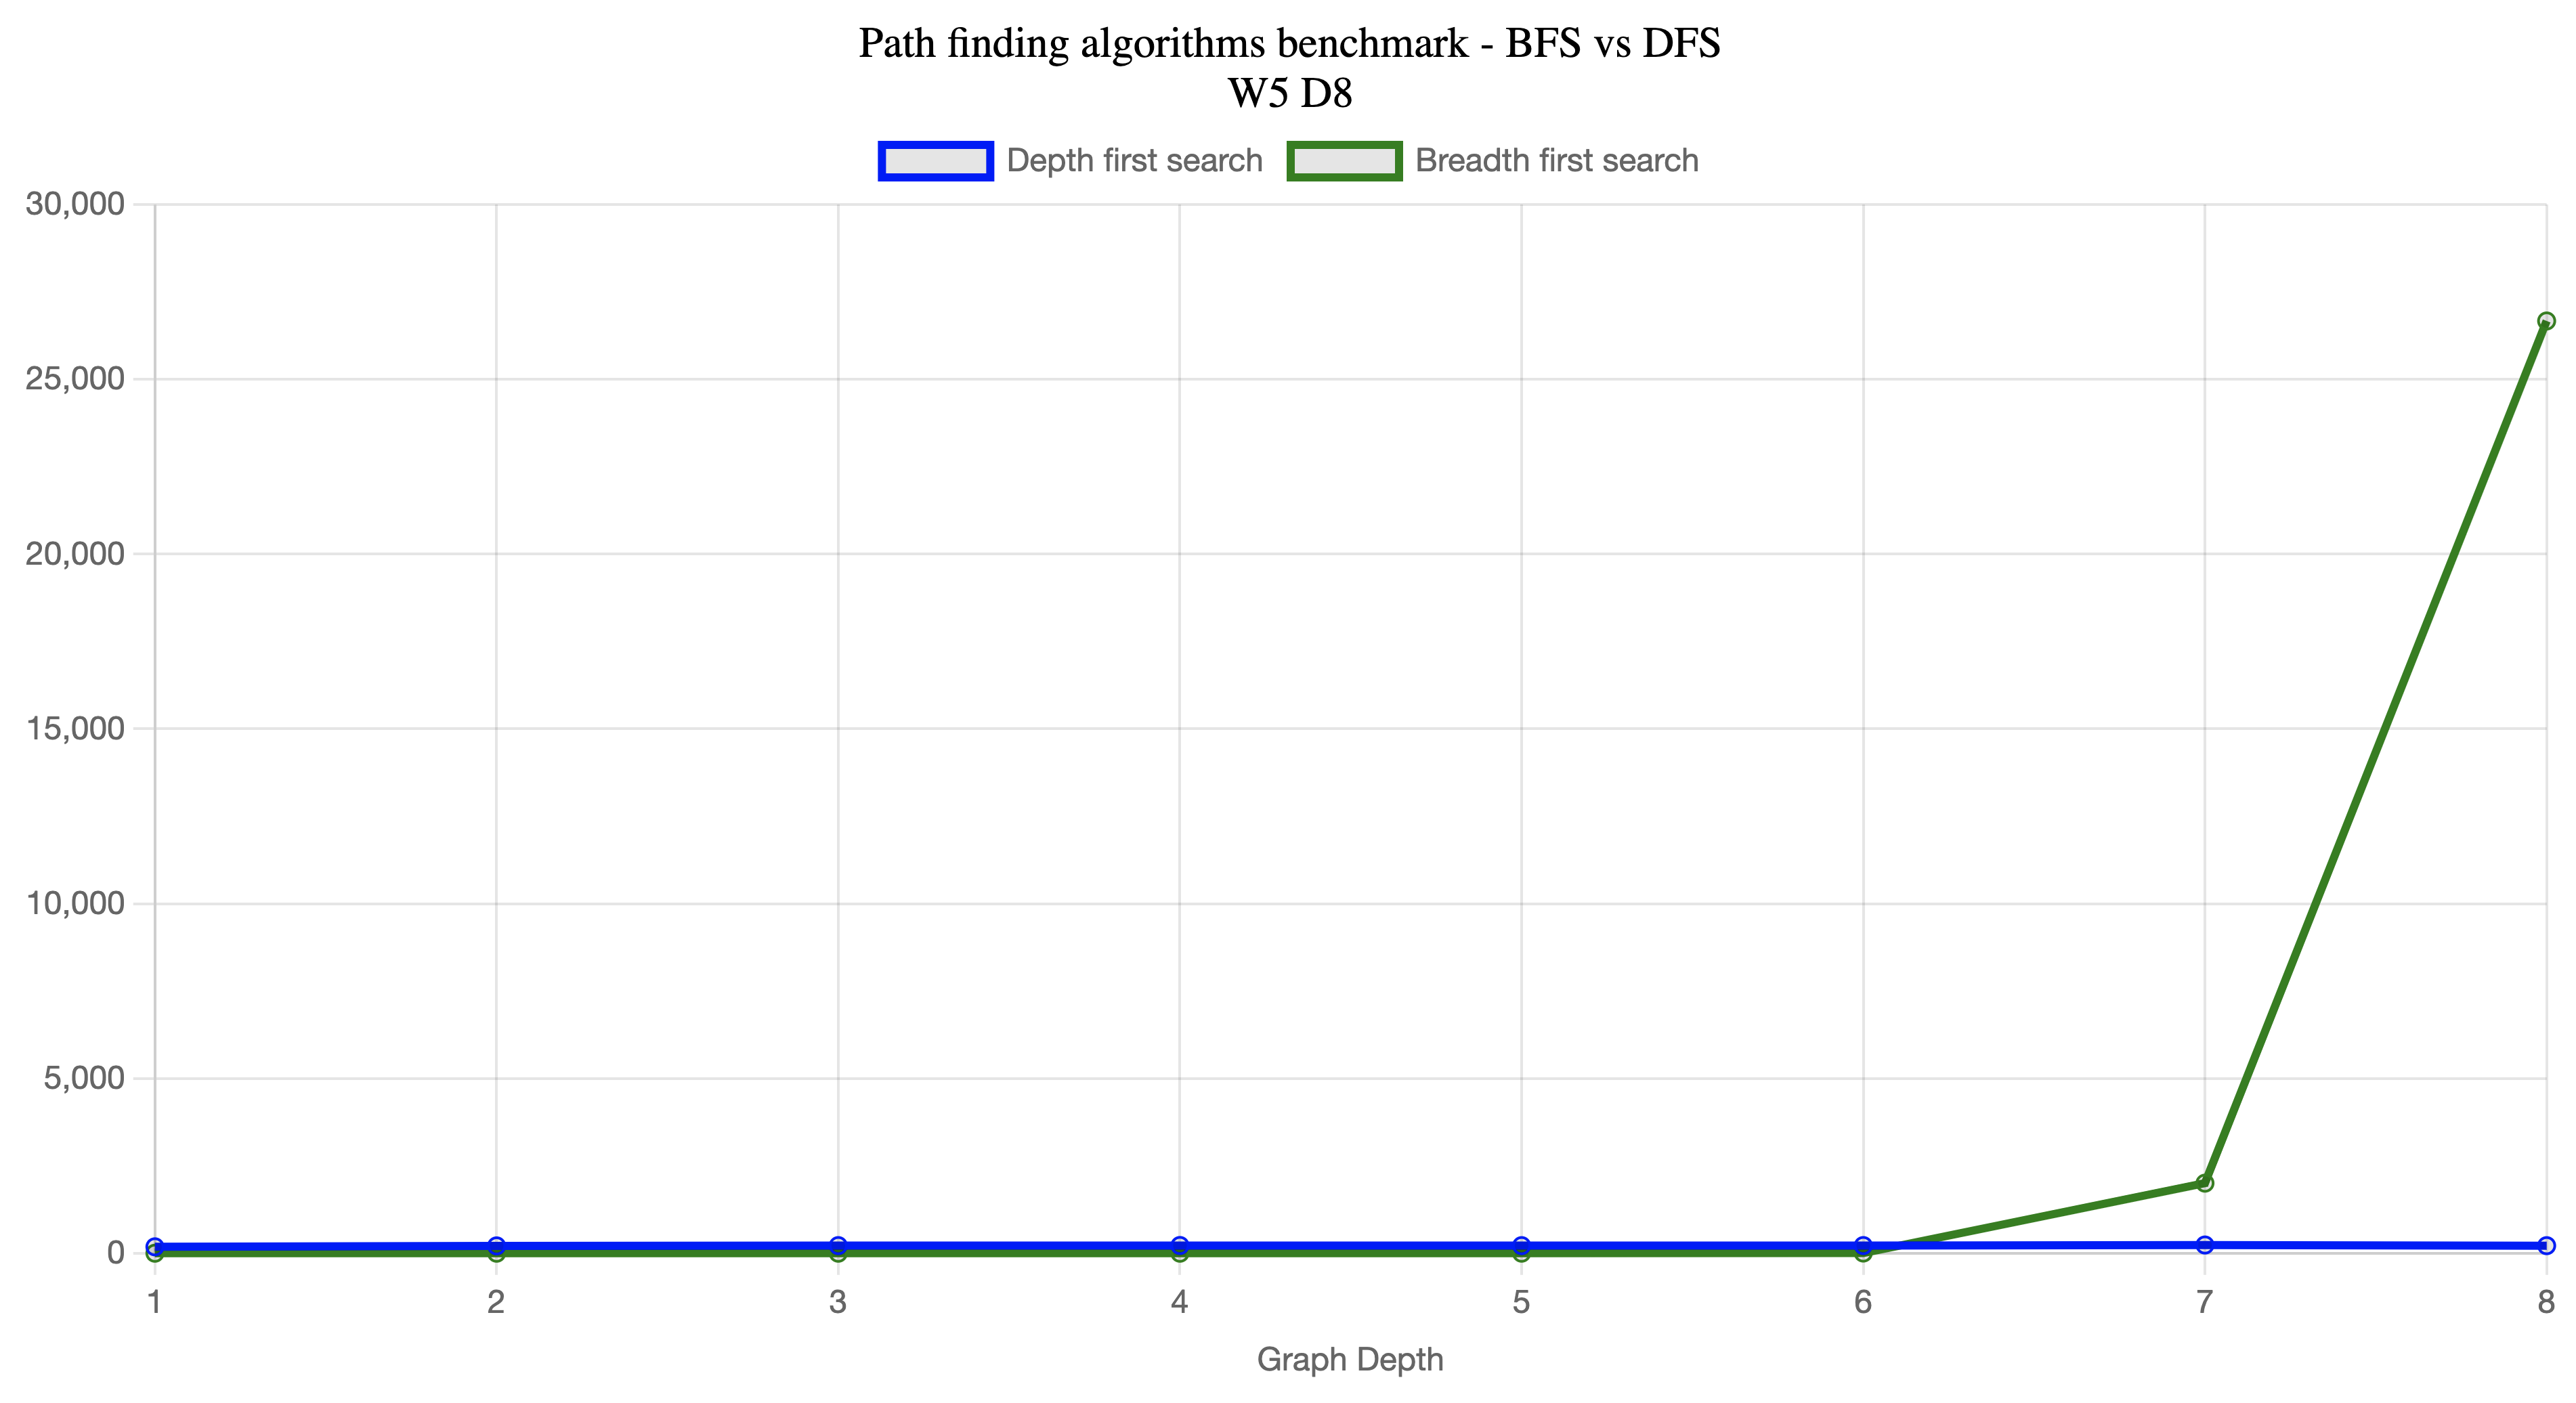
\includegraphics[width=1\textwidth]{images/w5d8.png}
    \caption{Path finding comparison for a graph with width 5 and depth 8}
    \label{fig:w5d8}
\end{figure}

\begin{figure}[h]
    \centering
    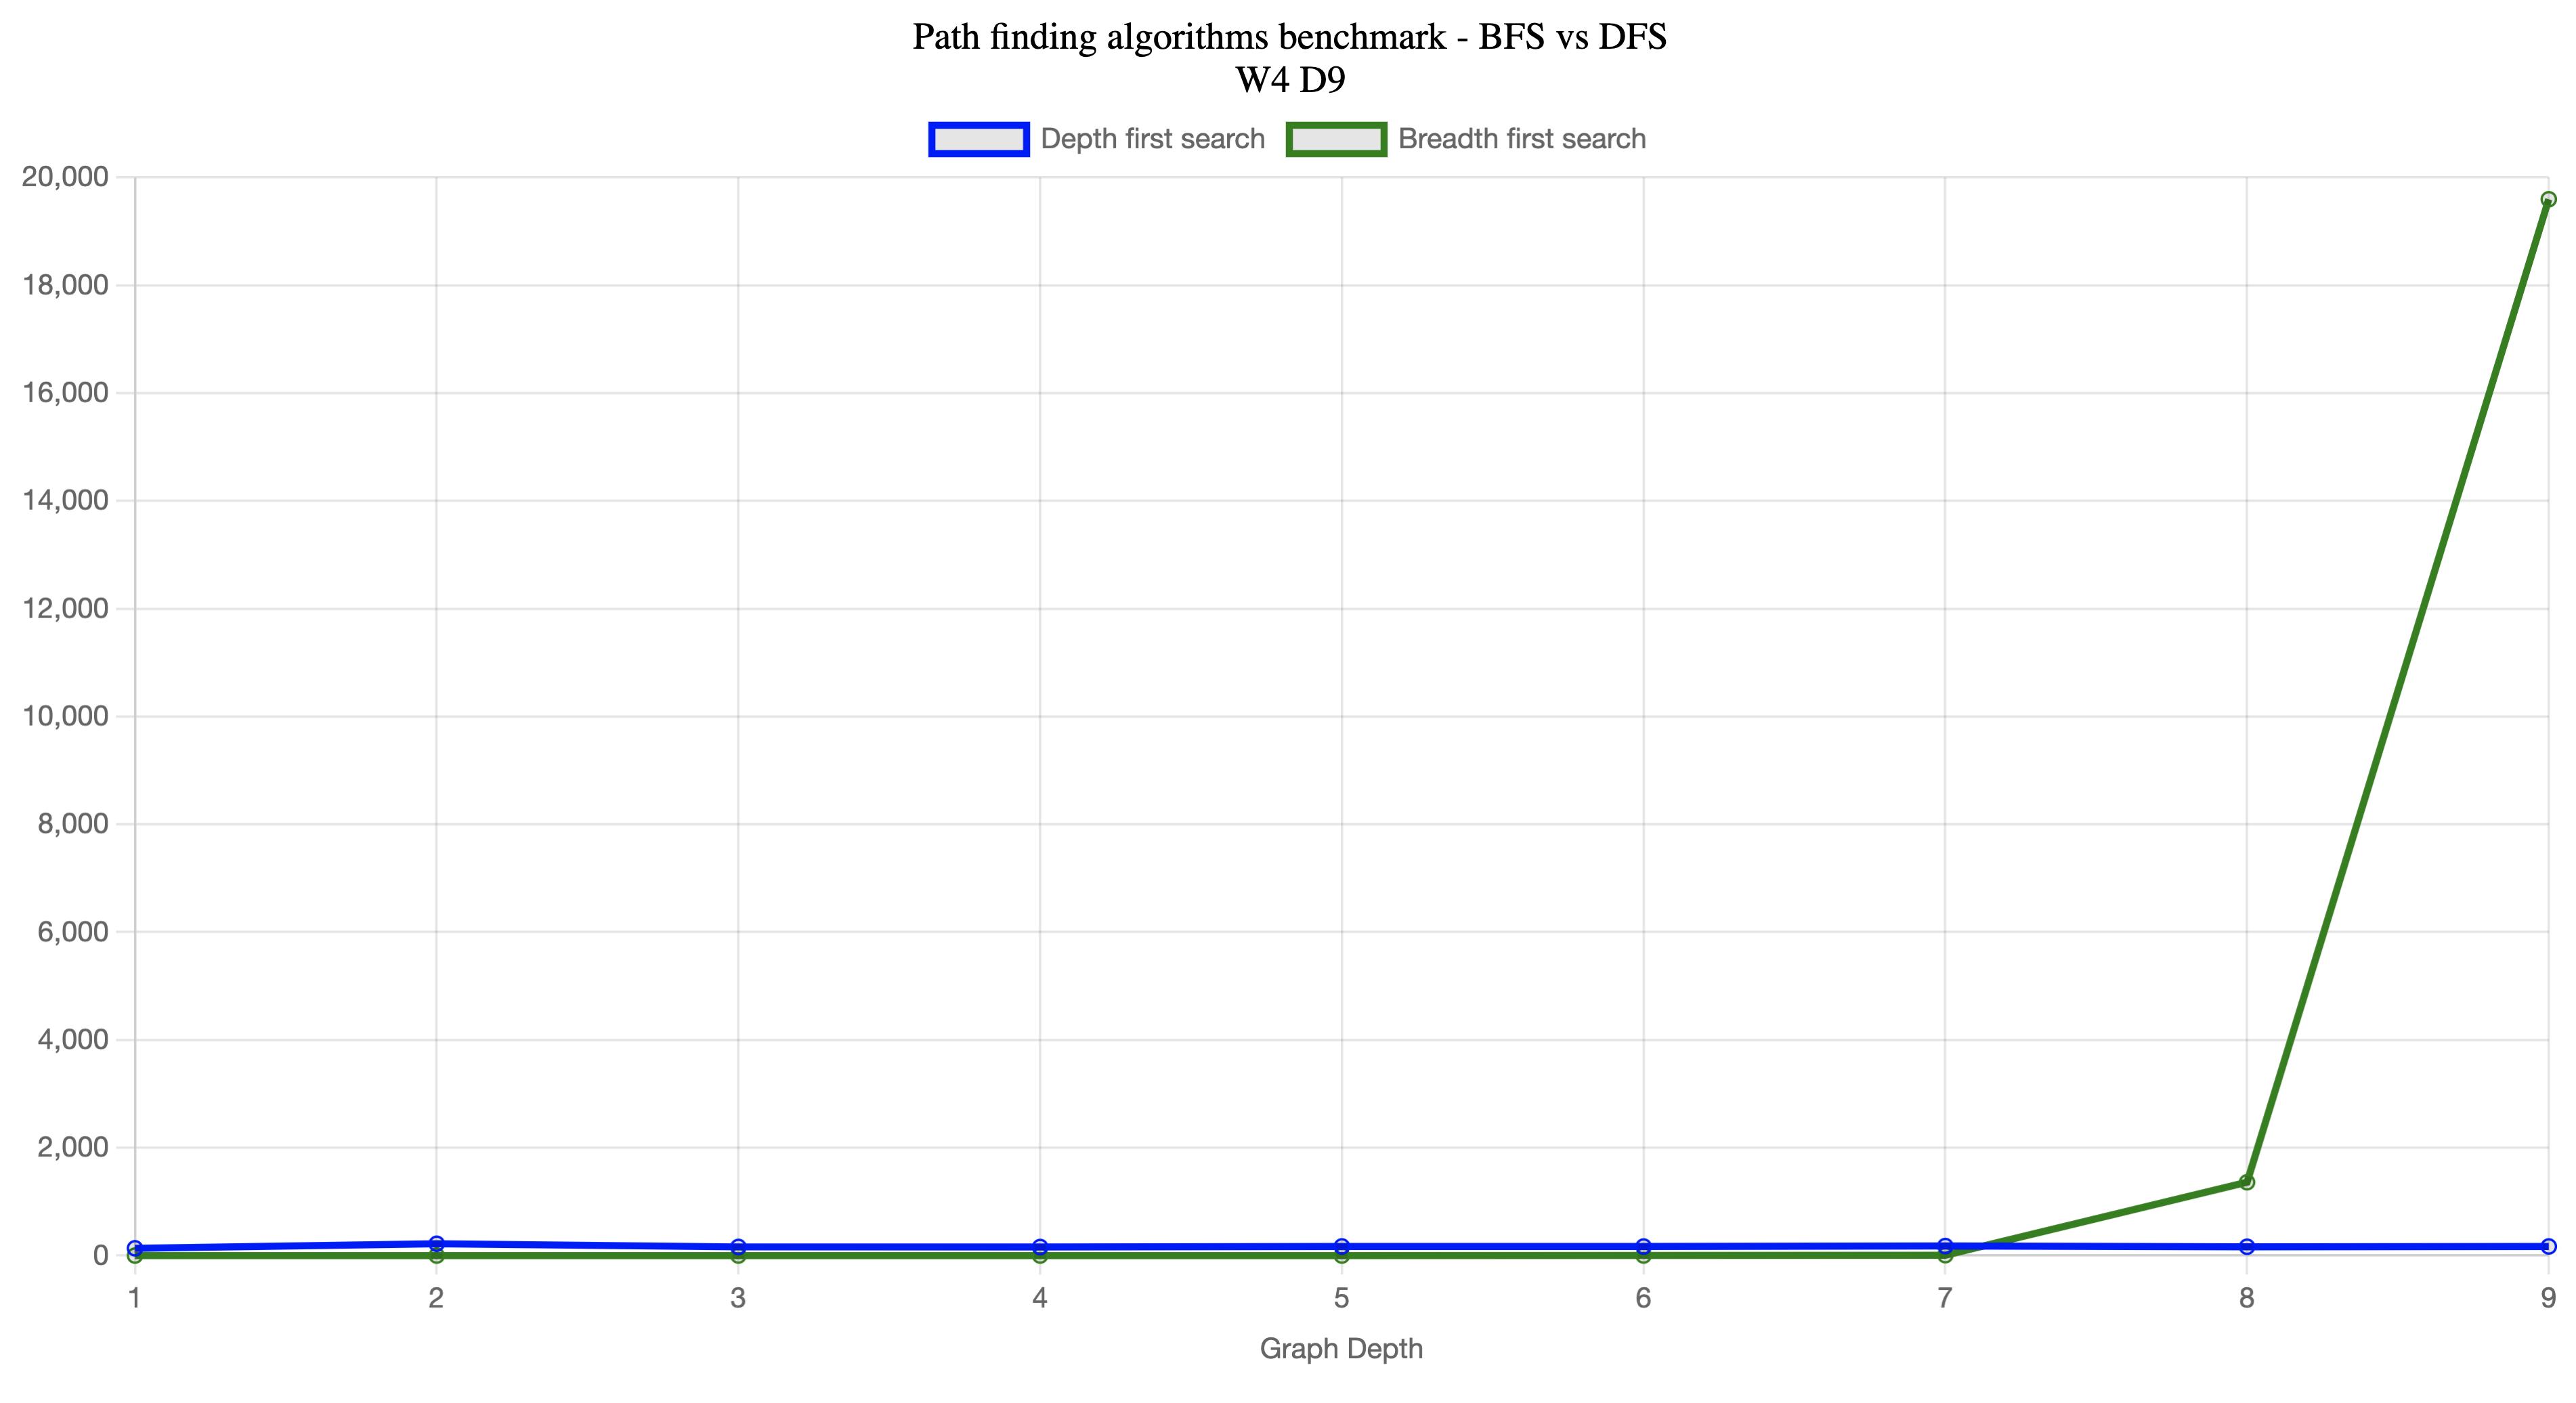
\includegraphics[width=1\textwidth]{images/w4d9.png}
    \caption{Path finding comparison for a graph with width 4 and depth 9}
    \label{fig:w4d9}
\end{figure}

\begin{figure}[h]
    \centering
    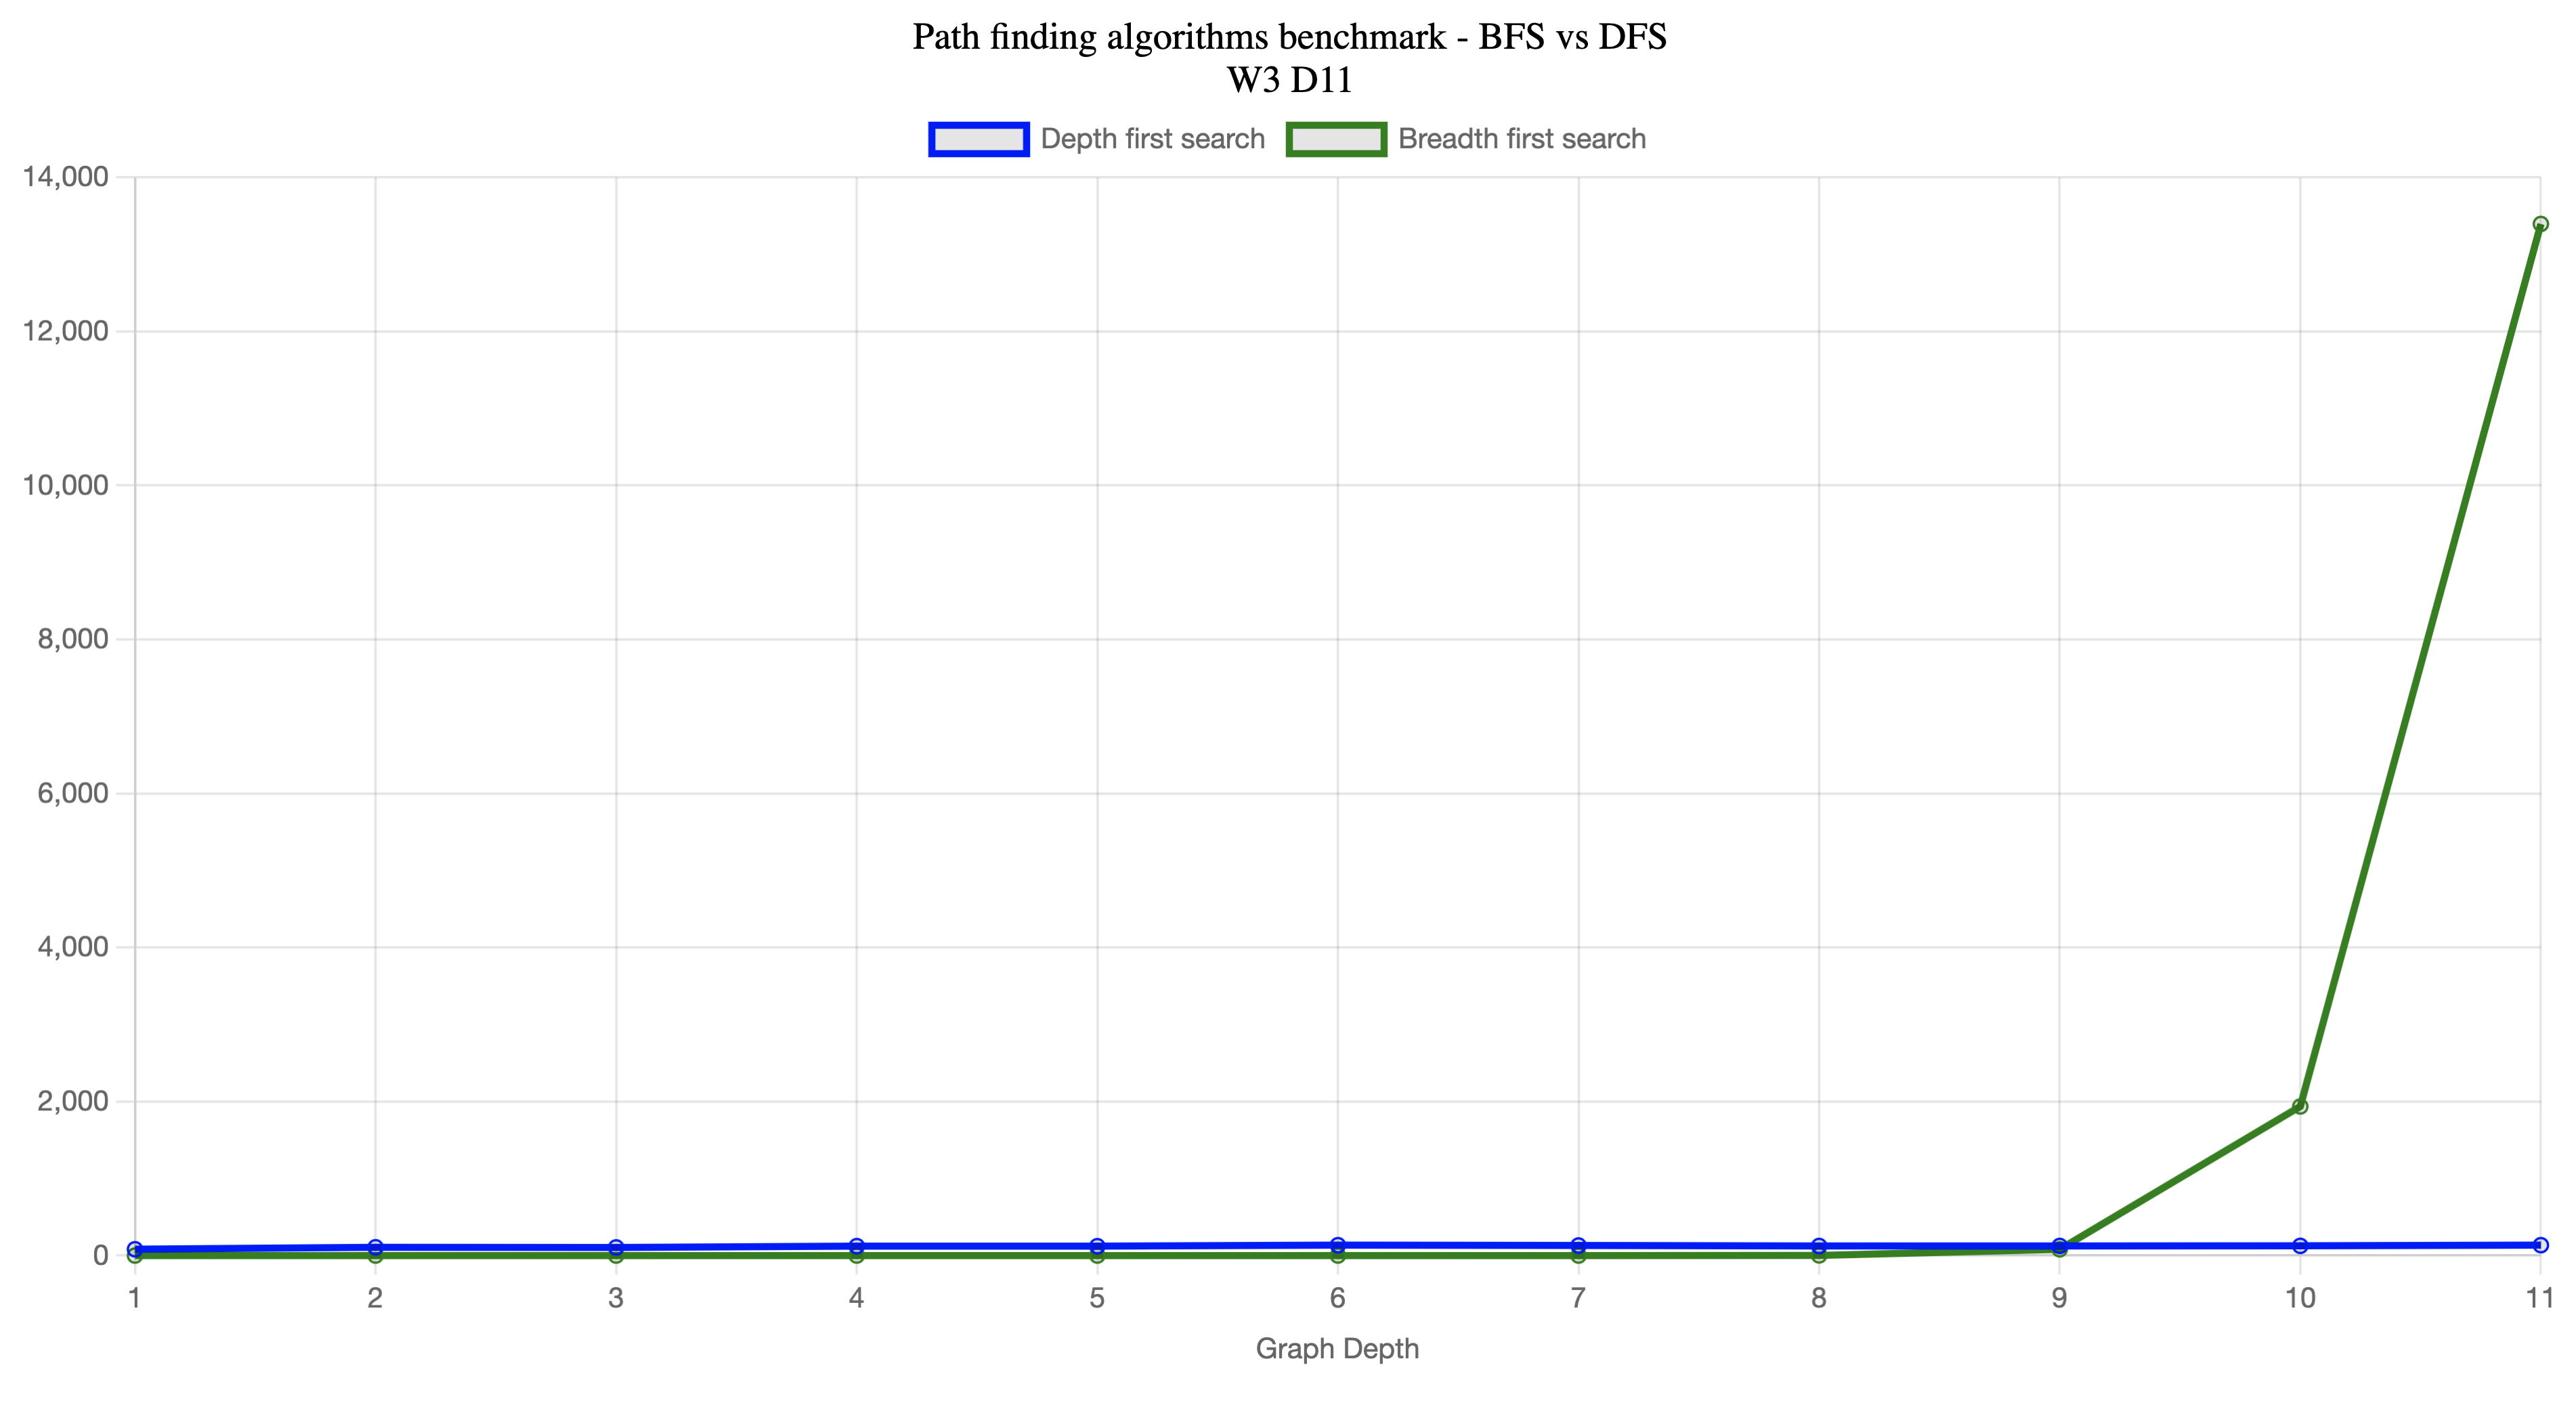
\includegraphics[width=1\textwidth]{images/w3d11.png}
    \caption{Path finding comparison for a graph with width 3 and depth 11}
    \label{fig:w3d11}
\end{figure}

\clearpage

As you can observe, the BFS algorithm works blazingly fast when the node is not very deep in the graph.

This happens because the of the principle according to which BFS works. 
It searches in the graph level by level, checking all the nearest neighbors.

DFS would have a chance to find the node, but because it dives directly into the deepest level
in graph it may perform redundant computations until it will procedd with searching in desired subtree.

Because of this particularities you can see how much slower BFS becomes as soon as the searched node 
is deeper in the graph. While DFS searches there, BFS still checks all it's neighbours

Even if the time complexity of both algorithms is:

$$O(n) = V + E$$

Depending on the edge case, one algorithm can be much faster than another.

\section*{Graphical Representation}
\hspace{0.8cm}
Graphical representation was done to showcase how the DFS and BFS algorithms would look on practice
and can be accessed online\cite{site}

\begin{figure}[h]
    \centering
    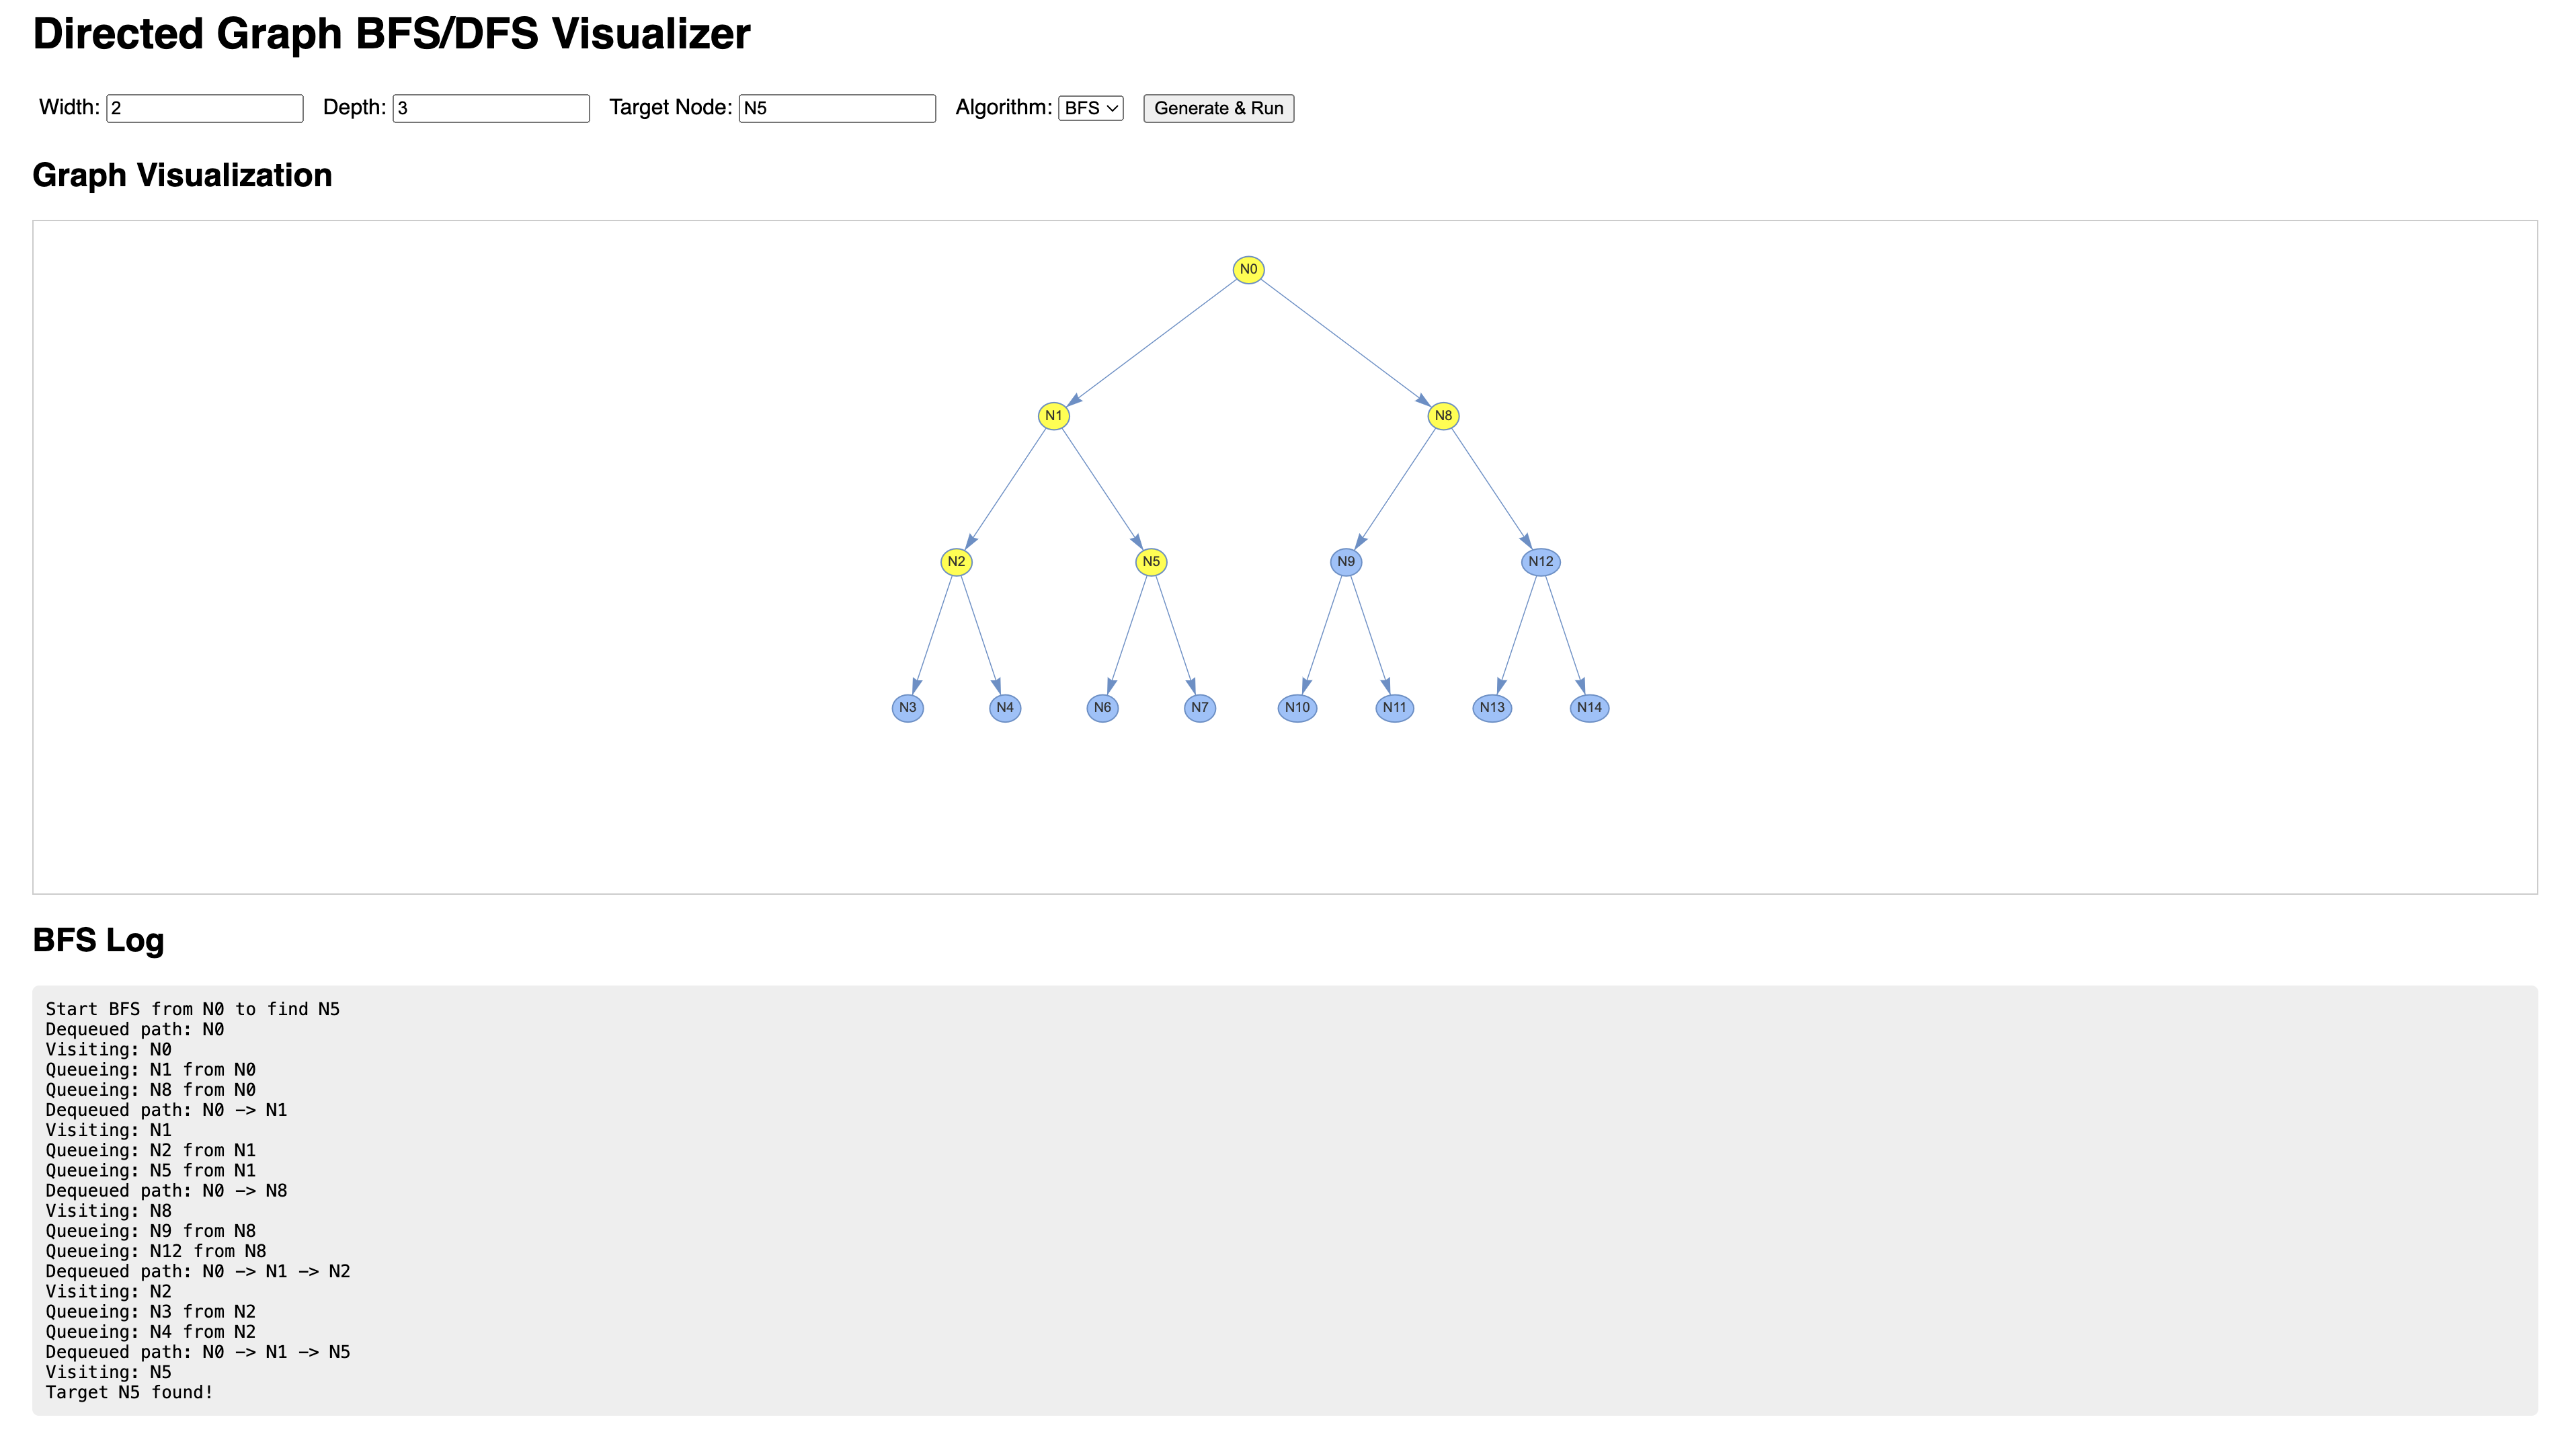
\includegraphics[width=1\textwidth]{images/site.png}
    \caption{Graphical representation of DFS and BFS}
    \label{fig:site}
\end{figure}

Here user have the following functionalities:
\begin{itemize}
  \item Choose the depth and width of the graph
  \item Chosing the node to search
  \item Switching between algorithms
  \item Display of the logs for each algorithm
\end{itemize}

\clearpage
\begin{thebibliography}{9}

  \bibitem{bytecoderef} \href{https://medium.com/dailyjs/understanding-v8s-bytecode-317d46c94775}{Franceska
      Hinkelman (2017) - Understanding bytecode \emph{Medium}}
  \bibitem{github} \href{https://github.com/DdimaPos/AA-labs/tree/main/Lab3}{GitHub repository of current laboratory work}
  \bibitem{site} \href{https://dfs-bfs-visualization.vercel.app/}{Graphical representation of BFS and DFS}
\end{thebibliography}
\end{document}
